\documentclass{acm_proc_article-sp}

\renewcommand{\rmdefault}{ptm}
%\usepackage[scaled=0.92]{helvet}
\usepackage{helvet}
\usepackage{courier}
\normalfont % in case the EC fonts aren't available
\usepackage[T1]{fontenc}
\usepackage{ifpdf}

%\usepackage[latin1]{inputenc}
%\usepackage[english]{babel}

%\ifpdf
%	\usepackage[pdftex]{graphicx}
%\else
%	\usepackage{graphicx}
%\fi

%\usepackage{subfig}			% to allow several sub figures

\usepackage{url}

\ifpdf
	\usepackage[pdftex,
		pdftitle					= {Urban Sketcher: creating urban scenery using multimodal interfaces on large screen displays},
		pdfauthor					= {Jose Pedro Dias},
		bookmarks         = true,				% do bookmarks
		bookmarksnumbered = true,				% keep sedtion numbers
	%	pdfpagemode       = None,				% start with closed bookmarks
		pdfstartview      = FitH,				% starting view scale
	%	pdfpagelayout     = SinglePage,	% one page at a time
		linkcolor					= black,			% links inside the document
		citecolor					= black,			% for cites
	%	linkcolor					= blue,				% links inside the document
	%	citecolor					= red,				% for cites
	%	urlcolor					= green,			% for urls
		colorlinks        = true]{hyperref}
\else
	\usepackage{hyperref}
\fi

\numberofauthors{2}
\author{
	\alignauthor Jos� Pedro Dias\\
	    \affaddr{Instituto Superior T�cnico}\\
	    \affaddr{Av. Prof. Dr. An�bal Cavaco Silva}\\
			\affaddr{2744-016 Porto Salvo, Portugal}\\
	    \affaddr{jose.dias@tagus.ist.utl.pt}
	\alignauthor Joaquim A. Jorge\\
	    \affaddr{Instituto Superior T�cnico}\\
	    \affaddr{Av. Rovisco Pais}\\
	    \affaddr{1049-001 Lisboa, Portugal}\\
	    \affaddr{jaj@inesc-id.pt}
}
    
\title{Urban Sketcher: Creating Urban Scenery Using Multimodal Interfaces on Large Screen Displays}
\begin{document}
\maketitle

%\def\hellow{
%	\textcolor{red}{HELLO!}
%}
%
%% with receiving param
%\def\hellow2#1{
%	\textcolor{red}{begin #1 end}
%}
%
%% alternative way of starting ending a command
%\def\hellow3#1{
%	{\bf#1}
%	\begin{bf}#1\end{bf}
%}

% show TODOs
\def\TODO#1{
	%\glossary{#1}
	\textcolor{red}{\textbf{TODO:} #1}
}

% hide TODOs
%\def\TODO#1{}


%%% ABSTRACT %%%
\begin{abstract}


% problem

A system was developed for the creation of urban scenarios produced on large screen displays
using laser pointers as input devices and supporting collaborative usage.
A novel interface had to be developed to support interaction with such input devices,
based on the concept of gates and circular menus with a non-intrusive interface.

% implementation / features

Users can navigate on a virtual world using a set of comprehensive navigation modes, namely:
first person, bird's eye view and examine modes, along with a multimodal flight mode controlled by speech commands and arm tracking.
Simple shapes can be created and modeled using a minimalistic set of modeling tools, defining a novel modeling interface.
Buildings can be instantiated from a library of facade styles by drawing
the desired blueprint and setting the facade height to generate unique buildings.
Additional styles may be implemented by making use of a developed XML format for defining fa�ade layout rules.
Buildings and other shapes can be transformed and cloned.
Objects in the scene can have notes attached to them to aid in reviewing sessions.
An alternative building creation work flow is proposed to take advantage of this system for early prototypes
and showcasing projects.
%
%The system architecture is described throughly, followed by implementation details and evaluation tests.
%It is shown that users could successfully make use of the offered features based on a stroke-based
%interface and set of comprehensive menus. 
%The project conclusions and future work close this document.

\end{abstract}


\keywords{
	stroke,
	building,
	multimodal,
	large screen,
	BREP
}


\section{Introduction}


% problem

With the advent of advanced visualization hardware it is now possible
to interact with complex representations of urban scenarios.
Systems capable of editing three-dimensional content
tend to be overly complex and make use of concepts
focused on mouse and keyboard interaction.
There's a demand for systems capable of offering 3D scenes rendering
and supporting multi-user interaction on large screens on fields
so disparate as architecture and the entertainment industry.

The current most common work flow process for defining the location and overall shape
of a new building is a process comprised of several discrete steps.
The architect starts by drawing rough sketches of the desired building.
These are highly subjective, with clients having a hard time in their interpretation and validation.
The architect then proceeds on studying the best location and orientation for the building.
This step used to be performed by observing 2D maps and on-site examination.
Once the location and overall building shape are defined, a rigorous project is drawn using
Computer Aided Design (CAD) software such as Autodesk Autocad\cite{SITE-AUTOCAD}.
This design is performed from scratch.
If architects are required to subsequently showcase the building appearance,
they rely on pre-rendered images and animations.


% related work intro

The state of the art in this domain was sought out. No project mapping the objectives of this project
has been developed though some, due to their dimension or common ground, were subject of analysis.
Work from other authors was reviewed when it addressed relevant problems, subject of usage on the project.
The most well known software bundles were compared to analyze possible solutions and avoid common mistakes.
A set of two interviews served as starting point for obtaining of both the current and desirable work flows
for cityscape creation, along with the definition of the main concepts the system was to support.


% challenge

Developing an application for such purposes requires dealing with several aspects
-- the large scale rendering of the scenario,
giving people means to interact with the screen,
allowing people to interact at the same time and
offering a simple interface adapted to the running environment.


% detail - laser / menu / gate interface

%The concurrent input of several users was handled so that each user
%could make the best possible use of the large screen area.

This system's interface was set for large screen displays and laser pointers chosen as the main source of user input
due to it being both portable and light.
The problem is that a laser pointer can't be tracked while the light is not turned on,
so any clicking behaviors are hard to mimic, even because users can't be 
precise while unable to view the laser pointer's projection on the screen.
An alternate interface urged to solve this issue, so instead of the commonly used buttons and drop-down menus,
crossable areas and ring menus were introduced.
To better explore the available space on the screen,
menus can be invoked as needed by performing preset strokes on the screen (gestures).

% important results

For every mappable feature, tasks were performed on both Urban Sketcher and other system - Google SketchUp.
Even though GSU relies on desktop concepts and input/output devices, users were able to perform the tasks
successfully and took less than twice the time performing them using such devices and interface.
Users easily learned the system's features and their menus, being able to easily
create 3D content such as buildings (template-based) and custom objects (using a tool set of simple modeling tools).


% main contributions

This project takes advantage of large screen displays,
made possible by the devised interface based on area activation and ring menus,
with users applying discrete strokes using laser pointers.
The navigation and shape creation functionalities focused on simplicity,
offering a set of tools and the capability to extend the software with additional scenarios and facade styles.
A novel set of modeling tools and interaction gestures was put to work, with emphasis on a multimodal flight navigation mode.
A new work flow was proposed so the system to be used both at early design stages and
when showcasing the project.


% mapa das estradas

%Following is the related work chapter where three existing solutions are analyzed due to their relevancy,
%along with a set of approaches other authors defined with might suit the application.
%A comparative analysis on commercial software bundles is performed to emphasize their advantages and avoid
%their flaws. The chapter ends with a summary of the obtained data after two interviews with architects.
%The design chapter is next, describing the broad view of the Urban Sketcher project, its architecture, modules
%and purpose. The concepts used throughout this document are defined here.
%Subsequently one can find the implementation chapter, where the various navigation modes are defined and
%justified, as are the content creation, editing and review features which make part of the system.
%A proposed work flow taking advantage of the system developed is then stated.
%The process of evaluation is described, presented and discussed on the evaluation chapter.
%This document ends stating the results which have been reached, the main contributions
%this project introduces and ways it can be enriched in the future.

%%% RELATED WORK %%%
\section{Related Work}

This section is the result of researching existing academic and commercial software systems and publications.
Since no prior systems with these requirements could be determined, related work was sought to cover subproblems
related to the design and implementation of such a system.

%The section starts by the revision of three academic solutions with common goals with the proposed solution:
%Arvika, Multi-User Tabletop Speech and Gestures and Digital Whiteboard.
%An analysis is then conducted regarding input and output modalities capable of enabling such scenarios,
%along with a set of shape creation and scene navigation techniques.
%A comparative analysis of commercially available building modeling software is then conducted.
%The section ends with the result of two interviews gathered with architects in order to survey
%building characteristics and possible improvements over the common architectural work flow.


\subsection{Existing Solutions}


% intro

Three systems will be discussed in this area, each one 
withstanding common goals with the idealized solution.


\subsubsection{ARVIKA, 2003}


ARVIKA \cite{ARVIKA} is a project with sponsoring from the
German Federal Ministry of Education and Research that was implemented between 1999 and 2003.
It focused on the development of Augmented Reality (AR) technologies to aid in performing industrial tasks.

An expert in the industrial area would carry a head-mounted display (HMD) with a camera mounted on it.
The real-time captured video was then interpreted and markers extracted from the image.
The camera's positioning and orientation were estimated and the HMD view was enriched with virtual objects
(see figure \ref{FIG-ARVIKA}, left).
The framework was distributed in the form of an ActiveX plug-in for the Internet Explorer browser
named ARBrowser.

\begin{figure}[htb]
		\centering
    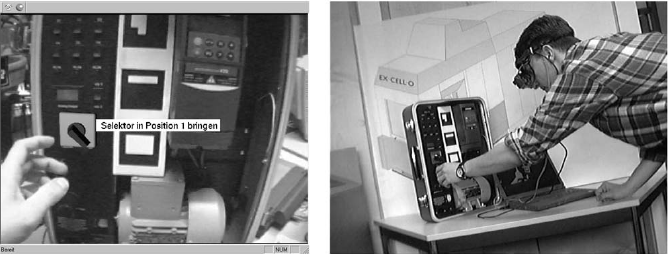
\includegraphics[width=0.8\columnwidth]{gfx/arvika.png}
    \caption{HMD augmented view; a user of the ARVIKA system}
    \label{FIG-ARVIKA}
\end{figure}


% discussion

Weidenhausen et al. \cite{ARVIKA-LESSONS} consider the deployment of the project as an ActiveX component
to be an advantage since it is based on a widespread program (Internet Explorer) and allowed developers
to create task scenarios with familiar technologies such as JavaScript and HTML.
Although the world's largest research project in the area, ARVIKA focused too much on the technical problems
regarding AR and little effort was spent on the creation of a suitable user interface.
The authors agree on a point: ``most people judge the usefulness of a technology mainly by its user interface''.
ARVIKA was meant to support many industrial scenarios -- development, production and services for several
industrial partners on different domains.
Creating a scenario was a time consuming task -- taking several days, according to Weidenhausen et al.
-- and required extensive knowledge in 3D modeling tools and VRML. No authoring capabilities were given to end-users.
This problem was identified as paramount and an authoring tool was scheduled for future development,
supporting generic task creation with parameters controlled by the users.




\subsubsection{Speech and Gestures on a Multi-User Tabletop, 2006}

Tse et al. \cite{SP-GEST-TTOP} developed a multimodal interface on top of Google Earth \cite{SITE-EARTH}
to be run on a multi-touch table.
The system allows multi-user collaboration with touch and voice commands.

The main problems found in adapting Google Earth reside in the fact that it was thought out as a single user program,
where only one action could be done at a time.
In this scenario several users could be disposed around the table with different orientations,
so text readability problems arose.
Additionally, user interface components such as the compass were placed at fixed points on the screen,
an approach that does not favor multi-user scenarios.
At 1024 x 768 resolution it was estimated that 42\% of the screen was originally consumed by GUI elements.
Since all users shared the surface, turn-taking had to be agreed by the users,
not being enforced by the system (see figure \ref{FIG-SP-TABLETOP}).
Most Google Earth interactive actions were mapped into gestures,
leaving the most abstract actions for voice commands activation.

\begin{figure}[htb]
		\centering
    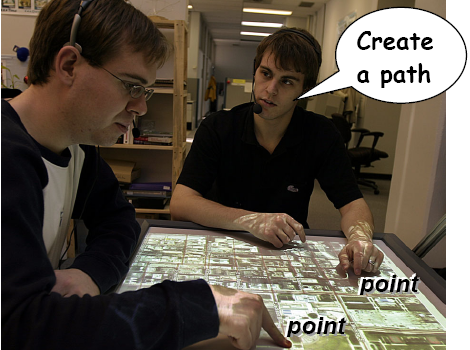
\includegraphics[width=0.4\columnwidth]{gfx/sp-gest-ttop.png}
    \caption{Two users collaborating on a Google Earth tabletop session}
    \label{FIG-SP-TABLETOP}
\end{figure}

This project shows the difficulties in adapting a production software thought out
for single user WIMP\footnote{Window Icon Menu Pointing device} interfaces for the support of collaborative scenarios.
A multimodal interface was built over the existing one, mapping most of its commands.
The set of obtained commands is a good example of how navigation can be performed on
3D scenery using a multimodal interface.
Google Earth is a good example of a navigation system suited for single user interaction.
It provides several functionality and could support the creation of buildings.
Making use of its large dataset of satellite images and topography would be excellent
for the target system.



\subsubsection{Digital Whiteboard, 1998}



Rekimoto \cite{WBOARD} created a digital whiteboard where each participant is given
a palmtop computer to handle. It works as a tool palette, remote commander, text entry box as
well as a temporary data buffer during whiteboard collaboration interaction.

The solution involves each participant carrying a pen and a palmtop,
with the pen working on both palmtop and whiteboard.
A direct manipulation method called Pick-and-drop(see Fig. \ref{FIG-WBOARD} left) was developed.
It allows a user to pick an object in his palmtop and dropping it on the whiteboard.
Text entry is performed on the palmtop and each user can choose the method he favors
(i.e.: handwritten recognition, soft keyboard, etc) for entering text.
No menus or tool palettes exist on the whiteboard -- they're available on each user's palmtop.
The main window is a multi page tool panel.
Users can store data elements in this window and paste them to the whiteboard
using Pick-and-Drop operations. (see Fig. \ref{FIG-WBOARD} right).

\begin{figure}[htb]
	\centering
	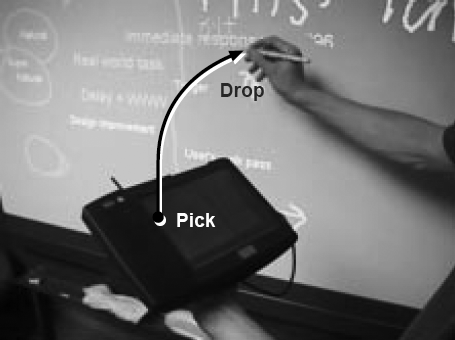
\includegraphics[width=0.4\columnwidth]{gfx/wboard.png}
	\caption{Digital Whiteboard: Pick-and-drop interaction}
	\label{FIG-WBOARD}
\end{figure}

Rekimoto concludes that by putting many functions on palmtops,
users tend to concentrate too much on their own palmtop devices,
degrading mutual awareness among the participants.
Pick-and-Drop often worked better than drag-and-drop,
particularly when user had to move objects for a long distance.
Drag-and-drop forces a user to keep the pen tip in contact
with the board during the entire operation,
a restriction not suitable for large display surfaces.

%\paragraph{Discussion}

%The solution where each user carries a palmtop for the creation of content such as note taking
%is suitable for an architectural design and review scenario.
%It grants the user the power to draw, type text or compose graphics 
%independently from one another and then replicating the information on the whiteboard.
%On the other hand there's the danger of users focusing too much on their palmtop and losing
%awareness of what's happening at the whiteboard.
%As result of this, a smaller interface device without all this functionality might be as suitable
%for interacting with a large screen, provided that these functionalities are offered by the interface.


%\subsection{Approaches}
%
%The set of available motion tracking techniques for gathering user input is discussed.
%The most common setups for rendering virtual reality scenes are compared.
%The shape creation projects Sesame and SmartPaper are analysed and three scene navigation concepts are visited.

%\TODO{??}

%%------!!!-------%%
\section{Design}

This section describes the proposed solution, the various modules which take part in the system and each module's responsibility.
It also introduces concepts used extensively throughout the solution.


\subsection{Proposed Solution}

Urban Sketcher is a system capable of controlling a large screen display,
offering conventional laser pointers for users to be able to draw on the screen,
with multi-user cooperative control (see Fig.\ref{fig:screen}).
To meet these goals,
a novel user interface is introduced, supporting multi-user laser interaction,
free invocation and dismissal of menus and purpose-organized options for easy
learning and usage of the interface.
The interface is based on crossing areas and circular menus.
The heavy usage on such concepts drove the author to devise
new ways of executing actions such as creating and editing shapes and buildings, scene navigation and note taking.
Most actions span the lifetime of a laser stroke, making the system stroke-based.

\begin{figure}[htb]
	\centering
	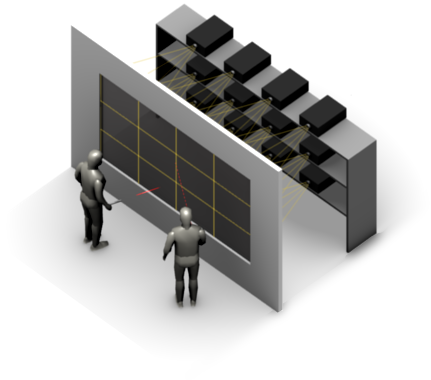
\includegraphics[width=0.6\columnwidth]{gfx/screen.png}
	\caption{Urban Sketcher interaction scenario}
	\label{fig:screen}
\end{figure}

\subsection{System Architecture}

Urban Sketcher is a distributed application -- it is composed of several modules which can run on different machines,
making use of a wired intranet network on the lab for the different modules to communicate.
The rendering infrastructure based on OpenSG computer nodes offers a cheaper solution for rendering large surfaces
while providing good performance. Most other modules benefit from a distributed environment --
tasks such as speech recognition, laser tracking and motion tracking benefit from dedicated machines due to their
heavy CPU processing requirements;
modules for integrating input modalities establish standard interfaces so they can be easily swapped by alternative media or integrated to other systems.
The core and middle-tier modules are modular mainly for abstraction purposes, dividing the complex problems of interface
and content management into manageable solutions.

%For easing up the development and flexibility, the system is able to run on a simple laptop machine with some of its
%modules disabled. On such setups the computer mouse generates events similar to the laser.

Urban Sketcher composed of a set of modules, most of them implemented as singleton classes
for managing subsets of the functionality. The interaction between system components is illustrated
on Figure \ref{fig:block-diagram}.
Modules implemented by the author are shaded blue, while integrated modules are shaded green.
A set of input adapters get data from several media -- laser strokes,
speech commands and motion tracked markers' coordinates.
These adapters generate commands which are consumed by higher level managers.

\begin{figure}[htb]
	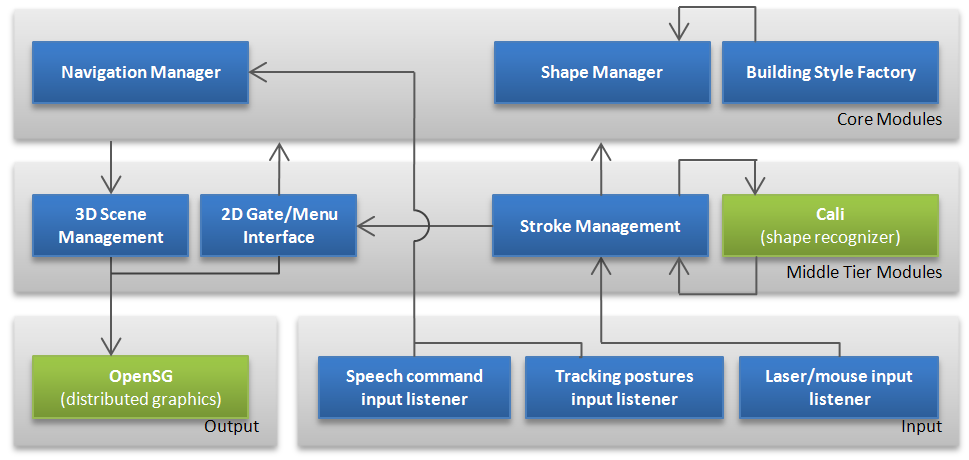
\includegraphics[width=\columnwidth]{gfx/charts/internal-block-diagram.png}
	\caption{Urban Sketcher Architecture Diagram}
	\label{fig:block-diagram}
\end{figure}

\textbf{Strokes} are managed and at low level, with key stroke gestures triggering commands.
A shape recognition engine named \textbf{Cali} \cite{CALI} was integrated to provide shape detection on two
types of strokes:
triangles, to invoke the main menu and
rectangles, to identify blueprint sketches over construction planes.
Cali is fed polyline information, returning the estimated recognized shape family and its parameters, if found.
The \textbf{2D Widget Manager} takes care of the visible interface, handling gate and menu events.

The \textbf{Navigation Manager} is responsible for keeping positioning information up to date.
It transforms the positioning state in response to actions issued by the supported navigation modes.

The \textbf{Shape Manager} holds the existing shape references and provides means for them to be selected and manipulated.
It caches loaded shapes to enhance performance in the generation of buildings, where attached geometry is bound
to repeat.

The \textbf{Building Style Factory} loads and parses style definitions into fa�ade-generating algorithms.
Once fed with blueprint information, desired style and height, this component is able to instantiate
a building and its details. Building details are attached shapes such as doors and windows, which makes the Building
Style Factory a consumer of Shape Manager.

The \textbf{2D Gate/Menu Interface} is a set of widgets and their logic, affected by strokes.
The widgets make use of the Model-View-Controller \cite{DESPAT} design pattern, with the controller ultimately making use of
higher level managers functionalities.
These widgets are oftentimes created by composition of simpler, general purpose widgets.

Both shapes and 2D widgets know how to render themselves using OpenSG, so they both interact with it.
\textbf{3D Scene Management} handles the representation of the virtual world and is controlled by both the Shape and Navigation
managers.

\subsection{Input/Output Communication}

\begin{figure}[htb]
	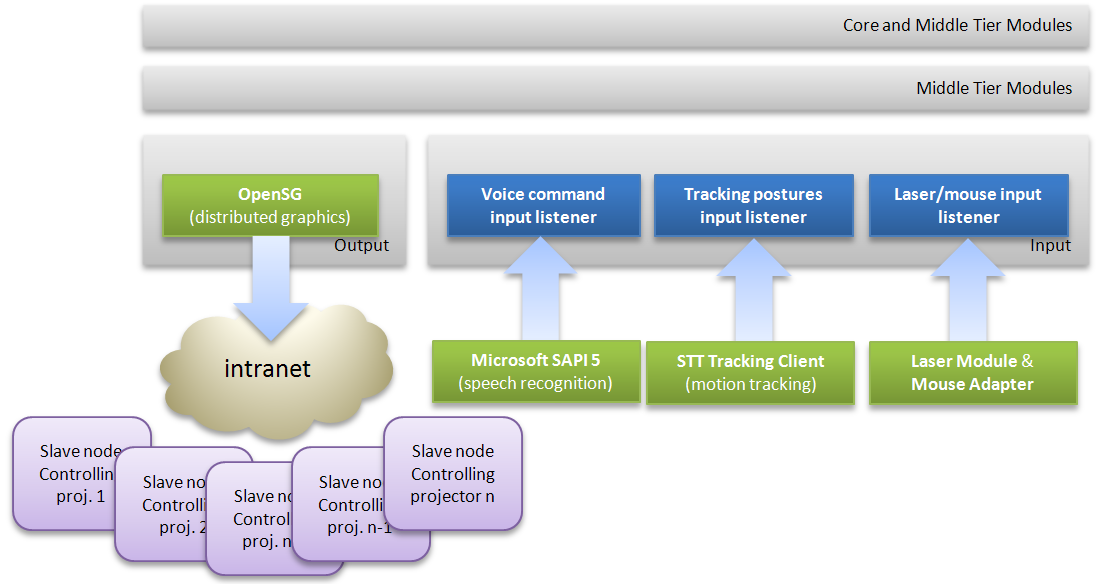
\includegraphics[width=\columnwidth]{gfx/charts/external-block-diagram.png}
	\caption{Urban Sketcher input/output Diagram}
	\label{fig:ext-block-diagram}
\end{figure}

Urban Sketcher gets input from the following media (see Fig.\ref{fig:ext-block-diagram}):
laser pointers, mouse input (for testing purposes) and optionally voice commands and tracking postures for
supporting multimodal navigation.
The system is able to render real-time views to any number of machines running OpenSG nodes.
XML configuration files allow parameterizing the range of affected machines and topology of the rendering slaves,
so rendering solely on the server, to a large screen display or both is a matter of switching configurations.

Both the speech command and tracking postures input listeners are fed by simple
applications of the available APIs from respectively Microsoft and STT.
STT is a hardware vendor of motion tracking systems and STT hardware was used during the development of this project,
along with various two and four camera tracking setups. Its software was used for calibrating the cameras and tracking
reflective markers.

The laser input listener receives data from the laser tracking module.
The laser tracking module obtains images from cameras mounted behind the screen,
with their lenses filtered for receiving infrared wavelengths, effectively isolating
the laser projections on the translucent screen surface. The contribution of all
laser projections sampled by the cameras are merged into screen space.
Since several users might be interacting simultaneously, a Kalman filter was used
to predict the path of each laser input and discriminate different strokes.
Development of the laser tracking module is work done by Ricardo Jota \cite{IMMIVIEW-EPCG}.

\subsection{Stroke-Based Input Interface}

This section details the concepts used for the implementation of the system user interface.

\subsection{Strokes}

A stroke is the result of continuous input from one laser pointer, from the time the laser
light button is pressed until it is released. 
By using the laser detection module the system gets a stream of laser readings which
come sequentially tagged, that is, the module identifies with reasonable success when different strokes
occur simultaneously, returning both readings tagged with different stroke IDs.
Even so, the module can't infer whether different strokes came from the same source laser pointer.
This limitation sets an important assumption in our system -- one can not know whether two strokes came
from the same user, therefore operations must take place during lifespan of a drawn stroke.


\subsubsection{Gates}

The most common activation action in current Graphical User Interface (GUI) computer interactions works
by displaying a button on the screen and the user activating it by pressing the pointer device's button.
Given that users will rely on laser pointers to interact with the system's GUI, a limitation derives from
using them instead of mice or track balls -- while a user isn't pressing the laser light button,
neither the system nor the user can accurately know where on the screen the laser is pointing to.
In order for the user to see the laser projection on the screen he must be pressing the button.
This system requires a different GUI solution.
Based on prior research by Apitz and Guimbreti�re \cite{CROSSY04},
the gate concept was implemented with slight changes.
The former idea was for actions to be activated by crossing an area by its explicitly drawn edges.
Some of the edges were red and other green, respectively enabling cancelation and confirmation actions.

The proposed gates work differently -- they're based on the action of crossing the middle of an area.
Gates have different visual states to suggest their internal state.
No edge representation is required -- once in the verge of crossing the center of its area,
the gate's visual representation changes into focused state and once the center is crossed it changes into activated state.
Gates in Urban Sketcher have mostly circular representations (when illustrated by icons), though
text labeled gates exist too when the content is of dynamic nature.

Internally a gate can be defined by an invisible line segment on the screen, bound by two visible extremes.
In order to activate it, one must draw a stroke which crosses the imaginary line segment, effectively crossing the gate
(see Fig.\ref{fig:activation}).
Gates can feature a text label or a suggestive image to symbolize the action they perform.
It was decided not to mix both representations to keep the interface uncluttered.
To help novice users to learn the function of each gate, a tooltip appears on gates when in focused mode,
that is, when approaching the gate's area of influence without crossing it. This way the tooltip can be read and the action optionally avoided.


\begin{figure}[htb]
	\centering
	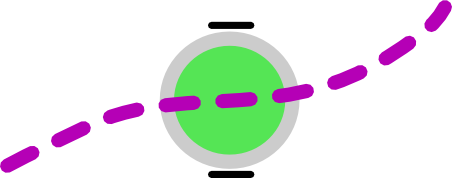
\includegraphics[width=0.25\columnwidth]{gfx/activation.png}
	\caption{Gate activation}
	\label{fig:activation}
\end{figure}


Though gates are a formally rigid concept, its implementation is just an approximation:
users can easily stay oblivious of these, keeping as bottom line the idea
of scribbling over the desired gate to activate it. 
With a set of distinguishable and clearly purposed illustrations such as those designed for the
Urban Sketcher system, gates can easily recognized and their purpose learned.
A gate can be repeatedly triggered for precision operations, as several gates can be sequentially
activated for achieving a complex state or action.



\subsubsection{Menus}

The menus of this system are ring-shaped, with its options spread along the ring in the form or gates.
The menu's background ring is translucent so the main viewport remains visible.
Different menus of similar functionality have the same background color to aid user recognition
(example: all navigation menus are green).
On the bottom-right area a curved label identifies the menu title.
The top-right area features additional gates for the dismissal of the menu, moving it around and
returning to the main menu if at a subsequent level (see Fig.\ref{fig:menu}).

\begin{figure}[htb]
	\centering
	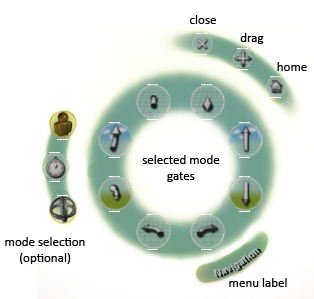
\includegraphics[width=0.45\columnwidth]{gfx/menu.png}
	\caption{Menu and its areas}
	\label{fig:menu}
\end{figure}

A lot of effort has been put for menus to be usable. On cases where menus offered a large number of actions/options,
those were clustered into modes to keep a conveniently small number of visible options.
On such menus, a set of gates at the left side of the menu represent the available modes.
Selecting a different mode is a matter of activating the corresponding illustrative gate.

Additionally to splitting menu gates into modes, gates can be grouped by purpose.
On shape manipulation menus, gates which share similar functionality are clustered into
general purpose action gates. As an example: move, move neighbors and extrude operations are clustered,
as are bevel and beveled extrude. This solution favors Hick's Law as stated by Landauer and Nachbar \cite{MENU-TREES},
since it shows a smaller set of easily distinguishable options, with the user setting the exact action
he intends to reach from a smaller, filtered set of gates.



\subsubsection{Stroke Gestures}

To invoke the main menu the user needs to draw a closed stroke resembling a triangle.
When such stroke is drawn one main menu instance appears centered on it.
Besides menus derived from the main menu tree -- which is invoked as we've just seen by drawing a closed triangle stroke --
there are menus which allow operating on existing shapes on the 3D world.
These are called contextual menus and they can be invoked by selecting a desired shape's face or edge.
To select a face one has to draw a small stroke starting and ending inside the face.
To select an edge one has to draw a small stroke starting on one of the edge's neighboring faces and ending at the remaining one, effectively crossing the edge to select it.

%\begin{figure}[htb]
%	\centering
%	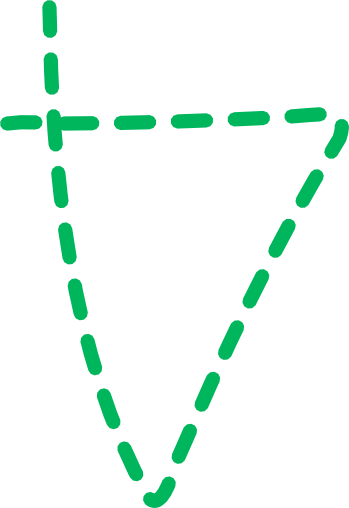
\includegraphics[width=0.15\columnwidth]{gfx/triangle.png}
%	\caption{Main menu stroke}
%	\label{fig:triangle}
%\end{figure}
%
%\begin{figure}[htb]
%	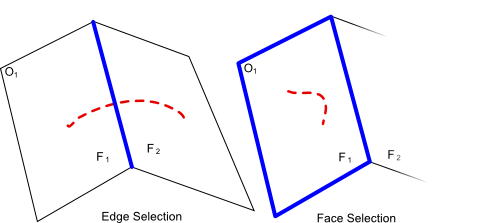
\includegraphics[width=\columnwidth]{gfx/face-edge-selection.png}
%	\caption{Edge and Face selection}
%	\label{fig:face-edge-selection}
%\end{figure}


%\subsubsection{Main Menu vs Contextual Menu}

Every action which generates new shapes is accessible from the main menu.
Actions which change existing contents are available from context menus for face and edge.
This segmentation rule was enforced so users know where to search when in need of an untried operation.


\subsection{Multimodal Input Interface}
\label{MMODAL-ITF}

Using laser input allows the usage of all system's functionalities.
Even so, an alternative arm-tracking and speech recognition command interface exists to enhance particular tasks.
The arms are tracked by attaching two reflective markers on each arm: one on each wrist and one close to each elbow.
Speech commands are obtained from a wireless headset attached to the user's ear (see Fig.\ref{fig:markers2}).


\begin{figure}[htb]
	\centering
	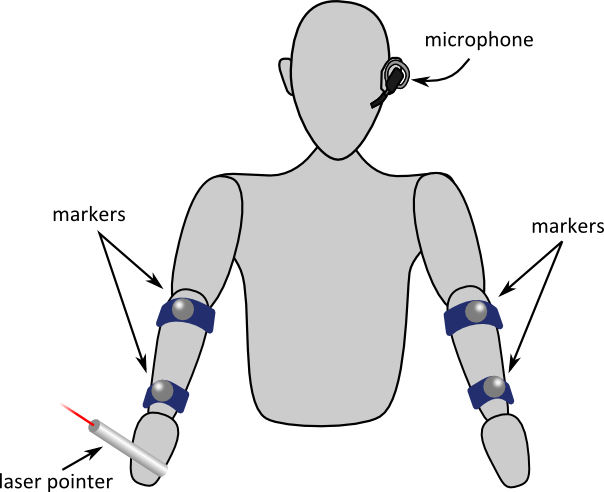
\includegraphics[width=0.6\columnwidth]{gfx/markers2.png}
	\caption{A user with reflective markers and wireless headset}
	\label{fig:markers2}
\end{figure}


\subsubsection{Content Creation Concepts}

The interaction between 2D menu based interface and the underlying projection of the virtual scene required a way of transferring
selected options to the scene and a dynamic way of specifying the parameters of a building so it can be easily created.
To provide such mechanisms to work, two content creation concepts were created.

%\subsection{Apply-to-Scene Creation}
%\label{design:apply-to-scene}

Several menus allow the selection of options (such as shapes or building styles), triggered from a menu.
The destination of such choice must be mapped into an object on the scene, therefore the concept of drag and drop was extended
-- the remaining of a stroke where such a selection is made server to point out the destination object, with the tip of the
stroke being the preview location while the stroke is taking place.

To create a new object on the scene one has to perform a stroke which activates the desired shape creation gate (cube for instance)
and continue the stroke onto the desired location where the shape is to rest. As soon as the gate is activated the shape appears
on top of the stroke and keeps following the stroke until it ends, offering a preview of the location where is would rest
if the stroke ended that particular moment (see Fig.\ref{fig:apply-to-scene}).
To figure out the actual location for the shape during the task the shape is iteratively collided against the
existing scene geometry so it stays in touch with the environment.

\begin{figure}[htb]
	\centering
	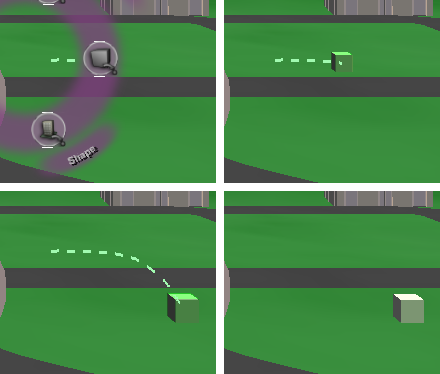
\includegraphics[width=0.7\columnwidth]{gfx/apply-to-scene.png}
	\caption{Apply-to-scene procedure - creating a shape}
	\label{fig:apply-to-scene}
\end{figure}

\begin{figure}[htb]
	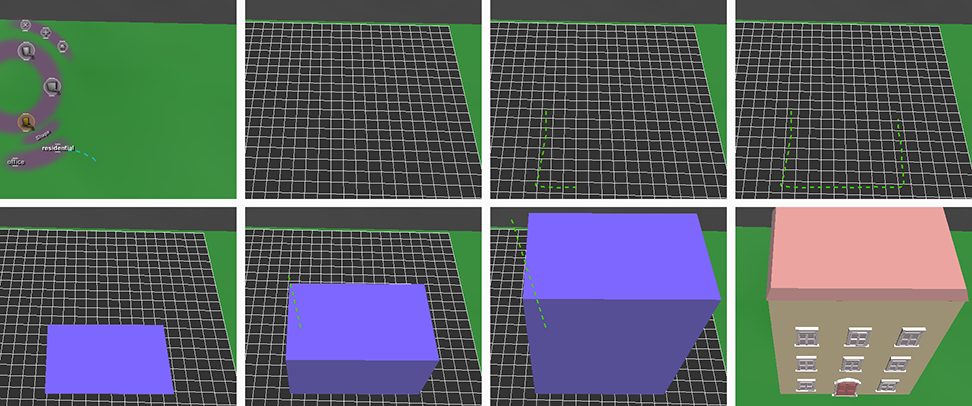
\includegraphics[width=\columnwidth]{gfx/building.png}
	\caption{Building creation procedure}
	\label{fig:building}
\end{figure}

%\subsection{Instancing a Building}
%\label{design:building}

To create a building one has to feed the system three parameters: building style, blueprint and height.
Due to the system decision for stroke-driven actions without global state, these three parameters are given with the
minimum strokes (two), as described next.
From a menu the list of supported building styles is presented to the user, each style a different gate.
Once activating the desired style the user starts an apply-to-scene process, moving a construction plane which must
be put where the blueprint is to be drawn.
The user draws a closed rectangle representing the blueprint and after closing it continues
the stroke upwards in order to define the building's height.
Once the stroke ends the building is generated according to the given parameters.
The construction plane has now carried out its purpose and therefore is terminated (see Fig.\ref{fig:building}).


\section{Implementation}

The execution of the projected features described earlier on is the focus of this section.
Functionalities are grouped by purpose and their details explained and discussed.
The several offered navigation modes, content creation and editing features and review features are described.
To close this section, an alternative work flow is proposed for taking advantage of the Urban Sketcher features.

\subsection{Navigation}

Good navigation modes are paramount for the success of any 3D based system.
The nature of this system, with the availability of a large screen,
stroke-controlled input and the aim of allowing unexperienced users to take control
of the system quickly, made this requirement even more relevant.

%According both to the task at hand and personal taste,
%several alternative modes may be useful to users.
%For tasks of simulating human movement, a \textbf{first person} based mode is expected.
%When searching for scenario features and moving big distances, a \textbf{top-down view} manipulation mode can be valuable.
%In occasions when an object is clearly the center of attention of the user,
%such as shape exploration and modeling operations, a \textbf{view centered on the object} mode is helpful.
%For giving an overview of the scenario and showcasing blocks of buildings, a high impact multimodal \textbf{flight movement} mode was developed.

The first three of the four mentioned modes were implemented with regular menu/gate widgets.
The flight mode is multimodal, relying on arm tracking and speech controlled input.

\begin{figure}[htb]
	\centering
	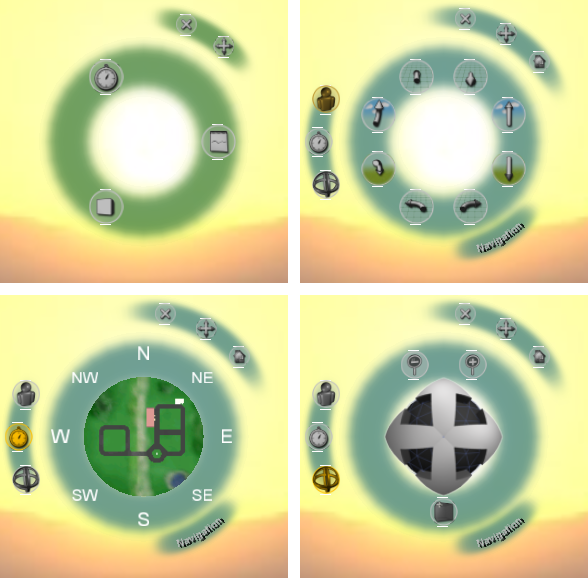
\includegraphics[width=0.8\columnwidth]{gfx/main-nav-menus.png}
	\caption{Main menu and all three navigation menu modes}
	\label{fig:main-nav-menus}
\end{figure}


\subsubsection{First Person Mode}

This first person navigation mode (Fig.\ref{fig:main-nav-menus}, top right) is centered on the current point of view and works by triggering the displayed gates.
It maps an interface resembling most first person shooters, offering translations and rotations around the current point of view (POV).
Such a mode is common on both games and modeling applications, so such mode is expected by users due to its familiarity
and good first-person-centered operators.

The First Person Mode features eight gates: four direction displacement gates and four rotation gates.
To stop the movement/rotation one can either trigger the gate again, effectively disabling the ongoing action
or by triggering a different gate action.
There are gates for moving forward/backwards, up/down, pitch up/down and yaw up/down
\footnote{The verbs pitch and yaw come from flight semantics: to pitch is to look up/downwards; to yaw is to turn relatively to the ground plane.}.

%The choice for this mode's layout suffered several evolutions.
%At early stages opposing directions where placed at opposite sides of the ring but this
%made correction by triggering the opposite action difficult, so opposing actions are now close together.
%In this mode a restriction of one enabled action at a time is imposed to keep the handling easy for novice users.

A helpful addition to this mode would be collision detection to keep users from crossing walls and the ground.
This could also help users moving on ramps and staircases.
The application of SmartCam \cite{SMARTCAM} would also enhance this mode,
at least the physics spring model simulation part.



\subsubsection{Compass Mode}

A birds-eye-view of the POV is helpful in 3D exploration scenarios,
allowing the user to better perceive the overall positioning in the world.
%An increasingly number of games feature a top-down view of the world.
%This system dues so too, not only for visualization but also for manipulation of the user's location and orientation.
The compass navigation mode was developed for that purpose (Fig.\ref{fig:main-nav-menus}, bottom left).
It allows the user to move along the ground plane and turn around it.
The compass navigation mode has two distinct areas:
the center circle displays a top-down view of the scene centered on the user;
the outer ring displays the main compass directions.
Dragging the center view translates the user along the ground plane while
dragging the outer ring rotates the POV, a concept easily grasped by test users.
The superimposed cardinal compass points are useful, particularly for people with a more technical background.

The Speed-dependent zooming \cite{SPEEDZOOM} could be applied,
translating drag velocity into exponential translation changes.

This mode could not be tested on multi-screen displays due to technical problems.
It was enthusiastically accepted on one-projector early tests, specially on users with a more technical background.


\subsubsection{Examine Mode}

When a program has the purpose of supporting the exploration of the shape of an object, an object-centric view is offered.
On simple scenarios the object occupies the center of the world and the view rotates around the world's center.
Urban Sketcher allows the center of attention to be dynamically set to any object of the world.

The examine mode features three gates and a center sphere (see Fig.\ref{fig:main-nav-menus}, bottom right).
The user is offered a gate so a new center of attention can be set. This action is performed by
activating the gate and ending the same stroke at the desired center of attention.
Once this is done, a spherical widget allows performing rotations around the object by dragging the sphere.
Two additional gates allow zooming in and out to reveal more or less detail, respectively.

For the users who got the grip of this mode, it has revealed itself a very efficient way
for both looking around and repositioning oneself.
Only laser-tracking problems inhibited a better use of repeatedly re-centering operation for movement.


%\begin{figure}[htb]
%	\centering
%	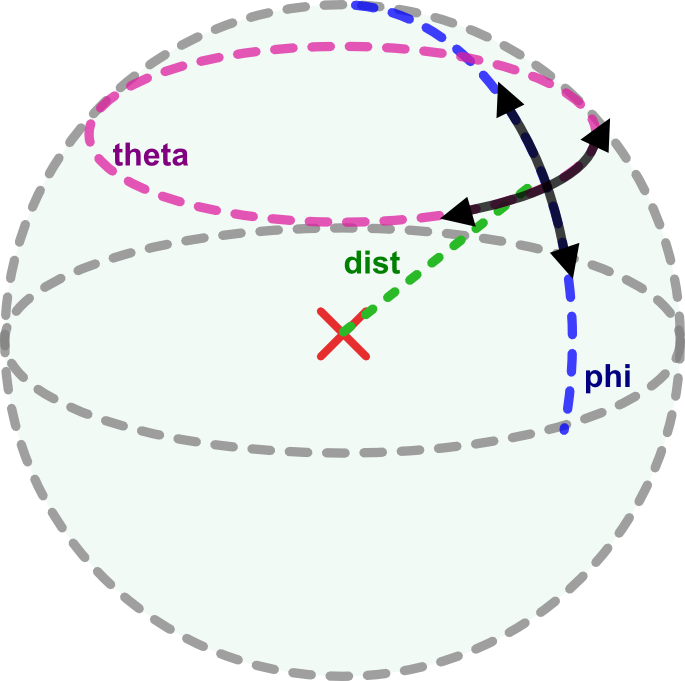
\includegraphics[width=0.3\columnwidth]{gfx/virtual-sphere.png}
%	\caption{Concept supporting examine mode}
%	\label{fig:vsphere}
%\end{figure}


\subsubsection{Multimodal Flight Mode}

The Multimodal Flight Mode is an alternative navigation mode devised by the author to provide an alternative way
of moving on the world.
This mode relies on arm gestures to control flight speed, rotation and altitude shift.
These operations are smoothly applied by continuous arm tracking and the application of a set of simple
rules to identify the user's purpose. This mode doesn't rely on laser input and can be enabled or disabled
by speech commands.

To implement such mode the \ref{MMODAL-ITF} Multimodal Input Interface was used.
Since it affects the point of view, this task can't be performed by
several people simultaneously, therefore unlike most of the system this navigation mode has global states
-- the user might be either stationary of flying (see Fig.\ref{fig:flight}).

The user starts interacting by having his arms extended toward the screen.
In order to begin flying the command ``Begin flying'' must be given.
To stop at any time one only needs to say ``Stop flying''
\footnote{Although semantically inconsistent, the words begin and stop were used after performing speech recognition
tests with both start/stop, begin/end and begin/stop commands, concluding that this combination had the better recognition ratio.}.

Controlling flight speed works by measuring the distance between hands -- the closer they are to each other the faster
the flight speed is. If the arms do a wide enough angle between them the flight comes to an halt.
Changing the flight orientation relatively to the ground is achieved by setting the arms angle with the ground at opposing directions,
with a bigger difference between these angles generating a faster rotation movement. If the user wants to turn right, for instance,
he has to raise the left arm and lower the right one.

To change flight altitude both arms must be oriented in the same direction relatively to the ground plane
-- either both raised or lowered. Again, the higher the angle is from the original forward pose position
the bigger the flight altitude shift is.

\begin{figure}[htb]
	\centering
	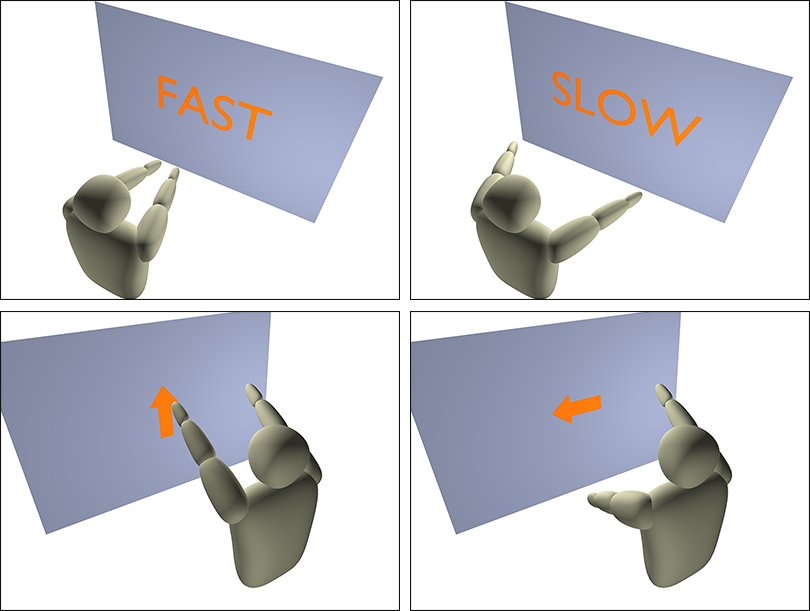
\includegraphics[width=0.65\columnwidth]{gfx/flight.png}
	\caption{Flight mode: controlling speed and direction}
	\label{fig:flight}
\end{figure}


%\subsubsection{Other possible navigational modes}
%
%In addition to the navigation modes made available in the system, the following modes might be of use.
%
%The multimodal ``go-to-here'' \TODO{REF}, with a combination of laser pointing to the destination
%and speech command to trigger the movement. This mode was requested on the final tests.
%
%The stroke-defined path, as suggested on the Path Drawing \cite{PATH3D}, discussed on section \ref{PATH3D-LABEL}.
%It would be useful to experiment this mode, but the requirements for its application were unmatchable:
%Igarashi's system uses a third person view with explicit avatar rendering. Moreover,
%Urban Sketcher stroke-based interface makes it hard to map a movement path stroke
%-- this would require multimodal integration with a ``move-like-this'' speech command.
%
%During the navigation tests at Glasgow, users suggested the addition of a list of recorded locations.
%The idea was for the user to get to a new and relevant point of view, such as a good fa�ade angle,
%and trigger the record location action.
%Recorded locations might be tagged by either speech recognition (example: ``record location \textbf{stadium front} now'')
%or scribble text recognition. Later on resuming to the saved location would be a matter of invoking the metadata
%recorded earlier.



\subsection{Creating Content}

The system's interface offers three families of shapes which can be instanced on the scene:
primitives, a set of previously generated shapes and set of known building styles from which to create buildings.
Primitives are the most versatile shapes since they support face and edge manipulation operations.
All shapes support simple transformations and cloning.
One uses building styles to create buildings on the scene. A library of generated shapes such as
people and trees serve as assets to populate the scene with details.
Primitives can be instanced as is or as building ground for custom shapes.

\begin{figure}[htb]
	\centering
	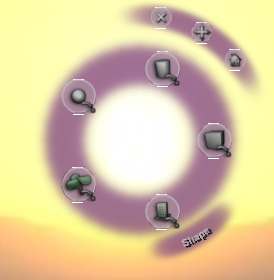
\includegraphics[width=0.4\columnwidth]{gfx/shape.png}
	\caption{Shape menu}
	\label{fig:shape}
\end{figure}


\subsubsection{Shape Internal Structure}

A shape in this system was implemented as a boundary representation (B-REP) \cite{REP-SOLID}.
This structured was used due to its simple translation to visual representation and
ease of shape modification.
To support several geometry operations an additional constraint was enforced --
all faces have four edges and therefore each edge has at most two neighboring faces.

The shape's surface is defined by two data structures:
an indexed array of \textbf{vertex positions}, used to store the position of each shape vertex;
an indexed array of \textbf{faces}, with every face being a counter-clockwise ordered set of four vertex indices.
An \textbf{edge} in the system is a pair of ordered vertex indices.
The ordering step makes the edge direction irrelevant for the edge definition, a desired feature.
Besides this information, each shape manages an auxiliary \textbf{edge map}.
This map associates a face to its bounding edges and vice versa.
The edge map allows efficient queries to be performed, such as:
\textit{which faces are bound by edge x};
\textit{what is the opposite edge of edge x in face y};
\textit{which other edges beside edge x make part of the face loop}.
These are all relevant queries for the implementation of internal shape operations.

Shapes offer methods to update their visual representation.
Shapes also make available a set of geometry modifying operations --
these are not only exposed to the user via UI, but also used by templates, as further explained.
In order to support undo operations, the memento design pattern \cite{DESPAT} was implemented.
A shape memento stores the internal structure of a shape at one point in time
and is able to restore that shape's state later on, if so requested.
A shape has a stack of mementos so multiple undo steps can be executed.


%\subsubsection{Shape Instancing}
%
%The instancing of shapes works using the Apply-to-Scene concept described on section \ref{design:apply-to-scene} Apply-to-Scene Creation
%and the respective Figure \ref{fig:apply-to-scene}.
%Every gate of this type has a small arrow running outwards as a hint to the user of this feature.
%The user activates the gate of the desired shape and ends the stroke where he wants it to rest.


\subsubsection{Shape Templates}

A template is a shape recipe with input parameters, defining a way of obtaining the desired shape
by applying a set of operations, with the passed parameters affecting the final geometry.
Templates are not directly exposed on the system UI. They're currently used solely to generate building ceilings,
but could be extended for other means.

Templates make use of shape exposed operations to generate the final shape.
For instance, the creation of a two-slanted ceiling starts from a regular box shape,
applying a sequence of two edge move operations.
%\TODO{EXAMPLE 2-SLANTED CEILING}
Additional templates could be easily created to aid in the generation of repetitive structures
such as railings and staircases.


\subsubsection{Building Style}

Buildings with the same purpose share most of their properties -- colors, floor height, fa�ade appearance, ceiling type, etc.
Such buildings differ the most on their number of floors and fa�ade dimensions.
To streamline the generation of building, the concept of building style was developed and implemented.
In Urban Sketcher a building is a complex shape composed of side walls, a ceiling and a set of attached shapes enriching the fa�ades with details such as doors, windows and balconies.

A building style is a set of rules and parameters, written according to a developed XML format. 
The system comes with a set of styles, with the user choosing the desired style to apply to the building he's about to create.
The building style factory is able to parse style definitions, instantiating and distributing attached shapes to make up
the facades according to the chosen style.
The building style grammar defines building parameters such as
floor-height, ceiling type and color intervals for the walls and ceiling.
It also defines a set of rules for the generation of the facade attachments that make up the final facades,
by grouping repeated structures, allowing random choice of facade elements and optionally have different layouts
based on floor number intervals or front facade.

%The building style grammar defines building parameters such as
%\textbf{floor-height}, \textbf{ceiling} parameters and \textbf{color-interval}s for the walls and ceiling.
%It also defines a set of rules for the generation of the facade attachments that make up the final facades,
%defined by the optional \textbf{front-facade} and the \textbf{facades} elements.
%
%One can define the layout of a floor with the \textbf{layout} element, composed of four sections:
%\textbf{left}, \textbf{center}, \textbf{right} and \textbf{other}.
%Of these only the \textbf{other} section is required and the layout works by trying to fill the facade space with \textbf{center}, \textbf{left} and \textbf{right}s' contents if those are present, repeating \textbf{other}'s contents for filling the remaining space.
%
%Inside these sections one can put any of the \textbf{us-element}s: \textbf{atom}, \textbf{group}, \textbf{sequence} and \textbf{random}.
%An \textbf{atom} is the simplest \textbf{us-element}, having the attributes
%\emph{type}, \emph{spacing} and \emph{height}.
%The \emph{type} parameter defines which shape to instantiate on the facade,
%\emph{spacing} how many length of the facade it will consume and
%\emph{height} can be used to shift the shape upwards (to move a window, for instance).
%
%The remaining \textbf{us-element}s allow combining \textbf{us-element}s.
%A set of \textbf{us-element}s inside a \textbf{group} create all content on the same place and measure the longest of its children.
%A set of \textbf{us-element}s inside a \textbf{sequence} create all children one after the other.
%The \emph{random} \textbf{us-element} is similar to \textbf{group}, but has the attribute \emph{odds},
%a set of comma separated ratios defining the probability of each child to be picked.
%
%Several floors can share the same layout. To apply a layout to one or a set of floors, the floor-span element exists.
%It can have either the \emph{at} attribute defined or both \emph{min} and \emph{max},
%resulting in the application of the enclosed layout to all the floors in the interval.
%
%One can also define a different facade style for the front facade with the element \textbf{front-facade}.
%This is useful when one wants to apply columns and doors to one facade but not the remaining ones.


%An example of a complete building style can be found on appendix \ref{residentialGrammar}. The resulting building is depicted on
%Fig. \ref{fig:style}.

\begin{figure}[htb]
%	\centering
	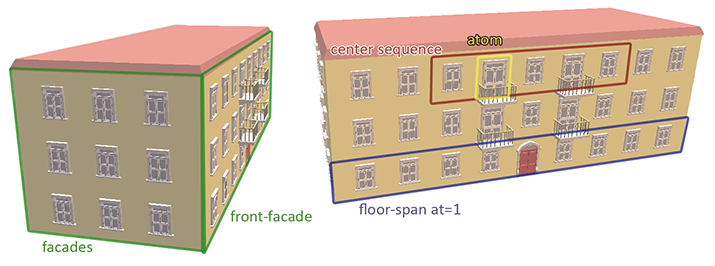
\includegraphics[width=1\columnwidth]{gfx/style.png}
	\caption{Generated building of residential style. Components highlighted for comprehension.}
	\label{fig:style}
\end{figure}


\subsubsection{Instancing Buildings}


Once the building parameters have been gathered by the interface, the building needs to be generated.
First the stroke is projected onto the construction plane and parsed by the shape recognizer as a rectangle.
The recognized rectangle dimensions serve as the blueprint which is extruded upwards for the measured height.
Then the building facades are generated according to the chosen style grammar and so is the ceiling.
The style grammar is fed each facade's dimensions and returns a set of spacings and facade elements that must be instanced
according to the rules defined in the style (see Fig.\ref{fig:style}).
To minimize the facade attachments in memory, a map of loaded attachments is managed so only the first instance of any
attachment is loaded.
%Appendix \ref{residentialGrammar} lists the residential style depicted above.



\subsubsection{Editing Content}

All shapes in the system are made of four-edged faces and all shapes are closed surfaces.
Operations such as the split by face loop rely on these properties.
Each shape computes each edge's neighboring faces (always two)
and therefore each face's neighboring faces, forming an auxiliary structure called the edge map,
used for optimized queries for neighbors.

%\subsection{Face and Edge Selection}

When a stroke finishes its start and ending points are projected onto the scene's available geometry.
If these two points lie on the same face of the same object that face is selected and the face contextual menu appears.
If the stroke start and ending points lie on different but neighboring faces of the same shape, the edge between
those faces is selected and the edge contextual menu appears.

%(see Fig.\ref{fig:face-edge-selection-imp} bottom).

%\begin{figure}[htb]
%%	\centering
%	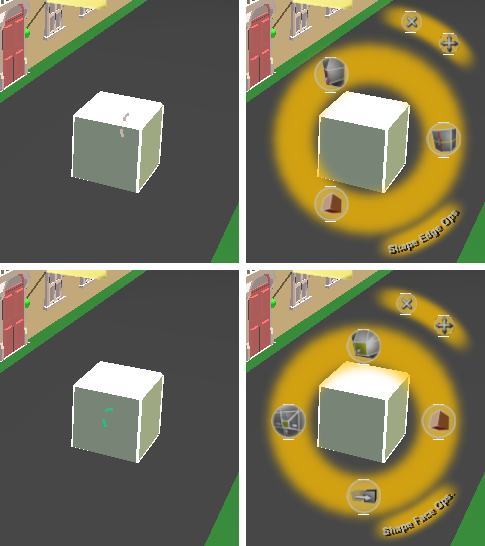
\includegraphics[width=1\columnwidth]{gfx/face-edge-selection-imp.png}
%	\caption{Edge and Face selection and their contextual menus}
%	\label{fig:face-edge-selection-imp}
%\end{figure}



%\subsection{Determining and Selecting Directions}
%\label{DIRECTIONS-LABEL}

In order to keep the interface simple and to minimize the number of steps needed to perform an operation,
a set of directions is estimated for edge and face selections
-- these are believed to be the most frequently needed vectors for shape operations.
When an edge is selected the computed directions are the edge outwards normal and the directions from the edge along its neighboring faces.
When a face is selected the computed directions are the face normal along with
the four directions from the center of the face to each of its neighboring faces.
If an operation requires the user to select a direction from the user the computed directions are displayed centered on the selected aspect
and color coded. The interface relies on the user to keep drawing the stroke after the operation is triggered so the remaining of the stroke data parameterizes the operation.

%\begin{figure}[htb]
%%	\centering
%	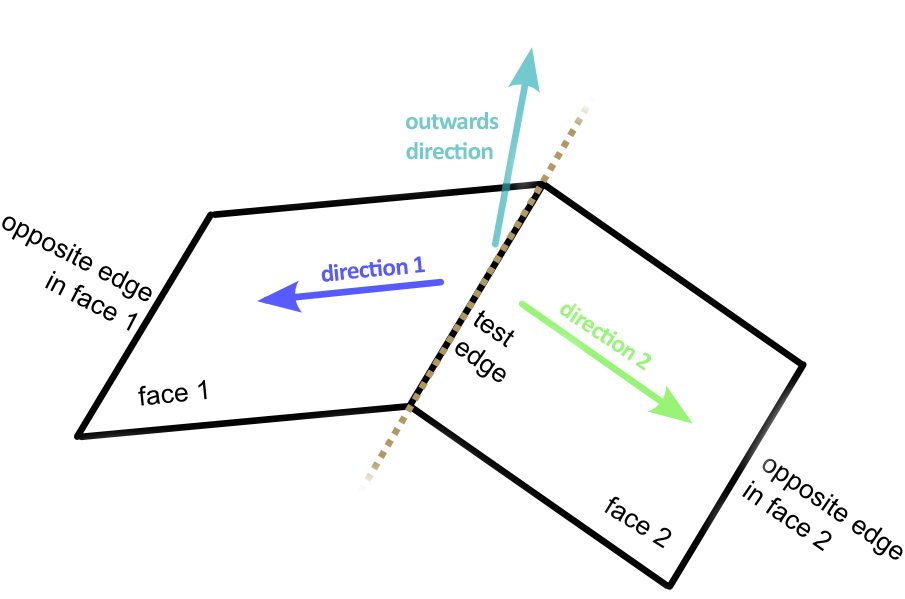
\includegraphics[width=1\columnwidth]{gfx/face-dirs.png}
%	\caption{Face directions}
%	\label{fig:face-dirs}
%\end{figure}


%\begin{figure}[ht]
%	\centering
%		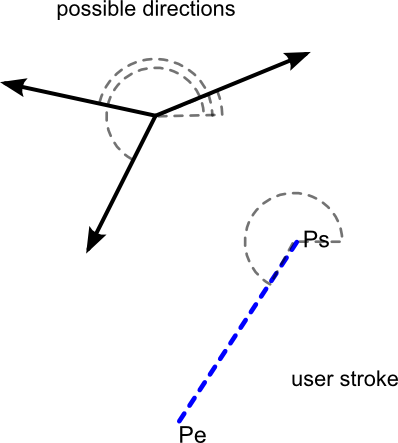
\includegraphics[scale=0.6]{gfx/election.png}
%	\caption{Direction selection}
%	\label{fig:election}
%\end{figure}




\subsubsection{Shape Operations}


This system has the goal of offering an easy yet reasonably powerful interface for modeling shapes.
The shape's internal structure was planned so both face and edge-based operations could be performed.
Every operation takes the triggering element (edge or face) as input parameter.
Most operations require additional information, obtained by extracting the user's stroke direction and length.
This interaction model keeps the number of stroke steps minimal while offering valid functionality for each operation.

The list of supported operations appears next, with them grouped by functional element -- the whole object, one of its
faces or one of its edges. Figure \ref{fig:ops} illustrates the application of these operations.

\begin{figure}[htb]
%	\centering
	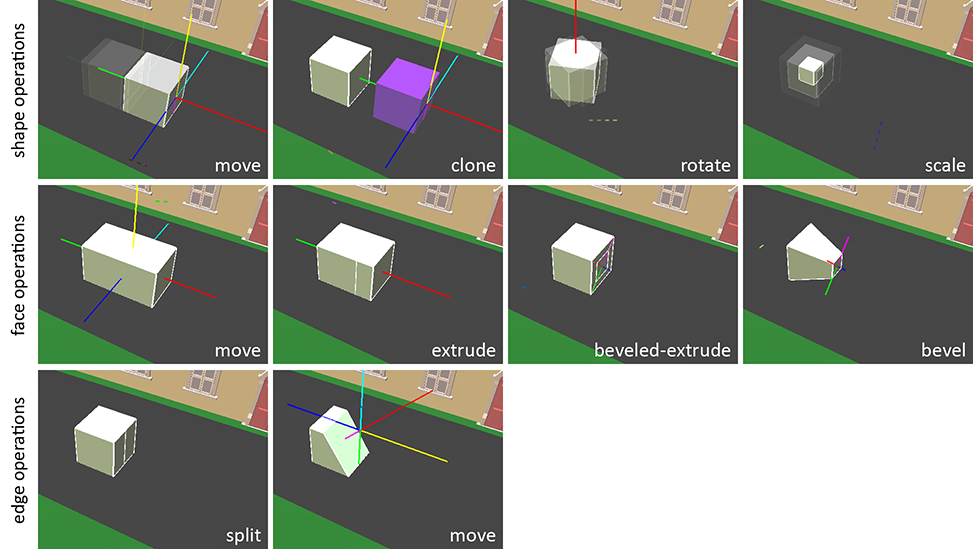
\includegraphics[width=1\columnwidth]{gfx/ops.png}
	\caption{Shape operation example applications}
	\label{fig:ops}
\end{figure}


%\subsubsection{Object Operations}

Available object operations are \textbf{translation}, \textbf{rotation}, \textbf{scale} and \textbf{clone}.
The \textbf{translation} operation accepts a delta vector, applying it in real-time on one of the five directions:
normal and the four surrounding edge directions.
\textbf{Rotation} and \textbf{scale} operations take only the stroke length --
scale transforms all three axes proportionally;
rotation can take the triggered face's normal as axis of rotation or can default to the YY axis for simplification,
since most urban changing operations make use of this rotation.
An additional object operation is \textbf{cloning}. The clone operation works like a regular translation,
leaving behind a copy of the original shape.
Since it uses the face normal and face-bounding edges' directions, the cloning operation allows efficient generation
of building blocks and repetitive structures.


%\subsubsection{Face Operations}

The \textbf{move} operation uses the same directions as translation, changing the position of the face vertices.
\textbf{Move neighbors} identifies neighboring faces having a smaller angle with the selected face than a defined threshold,
applying a move operation to the set of affected faces.
\textbf{Extrude} generates a new face for every face's edge and offers only the normal direction for moving the face outwards/inwards.
\textbf{Bevel} scales the face vertices, preserving inner angles.
The \textbf{beveled extrude} operation exists solely for convenience, generating a set of faces and applying an immediate bevel operation
to provide a simple way of creating relief details on faces for chimneys or windows.


%\subsubsection{Edge Operations}

Edges can be \textbf{moved}, with the offered directions being the edge normal and the opposite edges along the neighboring faces.
The \textbf{split along face loop} operation allows increasing the detail of a shape by cutting new faces along the center of the
implied edges.
On both edge and face context menus there's an option to \textbf{toggle} the visibility of the \textbf{shape edges}.


%\subsubsection{Possible Additions}
%
%The set of given operations offers a competent tool set for modeling simple shapes.
%During tests users have found several creative ways of modeling the requested shapes.
%Even so, multi-selection operations would be a nice addition to the tool set.
%In early prototypes of the system the closed lasso stroke was used to select multiple objects, which proved problematic
%since users inadvertently selected too many objects.
%Furthermore, using multi-selection for shape operations limited the direction seeking algorithms described above,
%which are key to the proposed simplified interface.



\subsection{Reviewing}

Notes can be created on the scene. A menu exists featuring a large area at the center where strokes can be drawn as if writing on paper.
A rubber option allows wiping the note contents. Once the note is written it can be attached to any scene object by using the
apply-to-scene concept (see Fig.\ref{fig:note}).
Notes are real 3D entities and can be hidden or edited by performing a closed stroke around them.

\begin{figure}[htb]
	\centering
	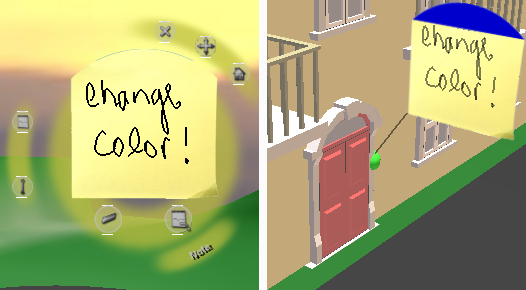
\includegraphics[width=0.7\columnwidth]{gfx/note.png}
	\caption{Creating a note and the result attached to a door}
	\label{fig:note}
\end{figure}


\subsection{Proposed Work Flow}

The proposed solution defines a system which allows architects to draft designs
directly on the 3D scene, allowing clients to better perceive the project at early stages
and empowering them with navigation and reviewing capabilities.
To accurately merge new buildings on the scenery one needs to obtain
satellite imagery and height maps of the landscape, a feasible task at present times.
Additional benefits could come later on by sharing the collected landscape information
with the CAD software and eventually exporting the draft buildings for reference.
Another benefit comes from getting a showcase platform for the project set up for free.
Instead of, or additionally to the set of pre-rendered images and short video clips,
clients now have at their disposal a real-time navigation platform which can be used
as a selling ad.

Shapes can be loaded or saved to XML and the simple descriptive format can be easily supported by 3D modelers.
For the purposes of the generation of terrains, library objects and facade attachments the Blender 3D modeling package
was used and an exporting plug-in developed.

%\subsection{Scenario Creation}

The system is a prototype tool so not much emphasis was put into the importing of content.
Even so, different scenarios could be created.
The height data from a terrain patch can be represented by either a height map or a topographic map.
With any of these data a 3D mesh can be generated - by vertex shifting a regular mesh for height maps or applying
a Delaunay triangulation to the contour lines.
With additional satellite imagery the terrain appearance could also be approximated by vertex coloring or texture projection application.


%\subsection{Building Style Creation}

New attachment shapes could be created using Urban Sketcher itself or an auxiliary 3D modeler.
Creating a building style is a matter of editing the style grammar, defining ceiling type, colors, floor height and most of all
the layout for the building floors using existing and/or newly created attachments.


%\TODO{UPDATED WORK FLOW DIAGRAM}
%
%\TODO{example stages}


%%% Evaluation %%%
\section{Evaluation}


The system has evolved with several user tests along the way.
During the course of the IMPROVE program several features were tested and enhanced.
The shape modeling operations, examine navigation mode
and building creation module were developed later on and were focus of the final user tests.


\subsection{Intermediate Tests}

% IMPROVE INTRO
Early stages of development of Urban Sketcher were supported by the European Union's
IMPROVE consortium \cite{SITE-IMPROVE}.
IMPROVE joined universities, hardware manufacturers
and design studios in the areas of architecture and car design.
Early prototypes of the interface and most of the navigation and reviewing functionalities
featured on Urban Sketcher
were developed during the period of the program. The interface, then called ImmiView,
was used for experimenting large screen display, tablet PC and head-mounted displays on tasks
of architecture design and reviewing sessions.

%IMPROVE was beneficial for the large brainstorming sessions which defined several of the concepts
%available today on Urban Sketcher, as with the series of User Tests which took place both in
%Glasgow Scotland and Lisbon Portugal.
%These tests served to get feedback on interface design and the
%navigation modes available at the time: first person and compass modes and the multimodal flight mode.

Several IMPROVE related publications were written as result of this project, such as  \cite{IMPROVE1} \cite{IMPROVE2} \cite{IMPROVE3}.
A more 
%\TODO{MORE IMPROVE. MAYBE INT TESTS SHOULD GO TO IMPLEMENTATION?}


%\subsubsection{Test Environments}
%
%The first Glasgow test occurred between the 16th and the 19th of April 2007 at the Glasgow Caledonian University.
%A hand-made screen frame was mounted and one infrared camera calibrated behind the screen.
%One regular XVGA projector was used with forward projection.
%
%The Lisbon tests took place between the 11th and 12th of June 2007 and focused on evaluating collaboration tasks.
%For these tests the Instituto Superior T�cnico Multimedia Lab was used\cite{LEME}. It has a structure of 4 by 3 projectors
%behind a translucent screen. The projection was performed from the back, with two infrared cameras mounted on the
%projector structure so a bigger portion of the screen could be tracked.
%
%The second Glasgow test occurred between the 16th and 19th of July 2007 at The Lighthouse building.
%This test was performed on a portable display and a projector set up for back projection along with one infrared camera
%for laser tracking.
%Four STT system cameras and reflective markers were used for tracking the user's arms.
%One Microsoft ZX-6000 wireless headset microphone was used to get the user's voice and the Microsoft Speech API 5.1
%American English version performed speech recognition to identify a set of commands issued by users.

\begin{figure}[ht]
	\centering
		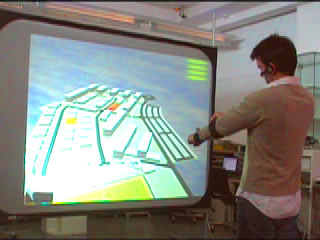
\includegraphics[scale=0.75]{gfx/don.png}
	\caption{A user performing multimodal flight during the Lighthouse test}
	\label{fig:don}
\end{figure}


%\subsubsection{Results}

The test at Caledonian University provided feedback about the first person and compass navigation modes.
The layout of the first person mode was changed as a result of this test --
its gates layout used to mimic the three axes for movement and had
rotation gates in between. These were changed to the cleaner design we have today.
The compass mode was enthusiastically adopted. It used to feature additional gates to move up/down and zoom compass view.
These gates were dropped to obtain a simpler design.
The Lisbon tests focused on testing collaborative tasks. Users were put in front of the screen and asked to work together
for the completion of navigation, annotation writing and object manipulation tasks.
%It proved the system could handle collaborative design and review tasks.
%\TODO{MORE?}
The Glasgow Lighthouse test focused on testing the flight navigation mode. One user had to wear four velcro fabric strips
with reflective markers and a wireless microphone. A 3 by 3 meters area in front of the screen was tracked by
motion tracking cameras.
%\TODO{...}



\subsection{Final Tests}

%\subsection{Objectives}

Most of the Urban Sketcher features were tested by handing out a set of vaguely
defined tasks for users to perform.
The largest possible subset of tasks was also performed on a well established software product.
For this matter, Google SketchUp (GSU) was chosen. GSU also denotes the aim of offering
a simple yet powerful interface. Even so, it is a desktop-based program and heavily relies on WIMP
concepts and mouse input.
Most tasks were successfully reproduced with Google SketchUp, with only the building creation task
absent for lack of supporting tools in the product for easy building creation and replication.
The point is to try obtaining reasonable times and expect US to overcome
many problems by the convenient grouping of actions in both the main and contextual menus,
along with the alternate method for applying operations on shapes and navigating the scene.


\subsubsection{Conditions}

The final tests were conducted months after the ones described above, with the system fully centered on Urban Sketcher
objectives and features. The most notorious features were tested in a series of small tasks: two for navigation,
two for shape modeling and one for building manipulation. To have reference data from which to compare to,
one of the analyzed systems on the Related Work section, Google SketchUp, was also used on the test.
Both the navigation and shape modeling tasks were performed on Google SketchUp -- building manipulation isn't supported by the system.

It is important to highlight that Google SketchUp is a commercial product with several years of development and
is based on familiar interface concepts and tested on a regular computer screen with keyboard and mouse input.
On the other hand Urban Sketcher tests are to be performed on a large screen display using a laser pointer
and an \emph{ad hoc} laser tracking system, with a set of novel interface concepts.


\subsubsection{Test Environment}

The final tests took place on the Instituto Superior T�cnico Multimedia Lab between the 28th of June and 1st of July 2008.
The tests were performed with the same environment as the Lisbon IMPROVE test described above -- a large display screen
of 4 by 3 projectors on a translucent screen. The laser tracking system was calibrated to get only laser information
from about 1/3 of the screen area. During the 4 days period they took place, 16 users performed the tasks described below.
Out of the user sample,
94\% of the users had college degrees,
31\% were women and the average user age was 37 years old.
This is a population with high levels of education. On the other hand the average age is of adult users,
not prone to new interface metaphors and with less precise motor skills.

User tests were performed individually and took between 60 and 90 minutes.
First a preliminary questionnaire composed of five close-ended questions was handed out and filled, to assert the past experience of users on topics of relevance.
Then the purpose of the project was presented along with a tutorial of Urban Sketcher's features and how to use them.
After a small hands-on period the tasks were given to the user to perform on the Urban Sketcher system.
Then a tutorial was given of the Google SketchUp program, focused on the features necessary to perform the tasks.
After a small hands-on period the navigation and modeling tasks were performed on the Google SketchUp system.
To finalize the test, the final questionnaire was handed out and filled. It was composed of 13 close-ended scaled questions
and five open-ended questions, the former to obtain feedback regarding the Urban Sketcher system and the latter
focused on comparing the two systems.



\subsubsection{Results}

During the tests, task completion times were measured in minutes and both user errors and system unexpected events were
logged. On table \ref{table-times} the summary of times for completing all the tasks is listed.
Chart \ref{graph-comparison}
is a box and whiskers chart, depicting the time users took to complete the tasks.
The whiskers define the range of sampled results, while the box ends mark the 25th and 75th percentile of the data.
The diamond marks the average value. Blue boxes were used on Urban Sketcher, gray ones on Google SketchUp.


\begin{table}[htb]
	\centering
	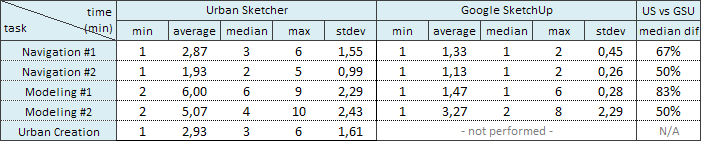
\includegraphics[width=\columnwidth]{gfx/eval/table-times.png}
	\caption{Task completion times on Urban Sketcher and Google SketchUp}
	\label{table-times}
\end{table}




Tasks performed on both systems were expected to show discrepancies in both completion time
and number of errors.
Most users are proefficient working with the mouse.
The \textit{ad-hoc} laser tracking system used in the test:
didn't map the whole screen;
had calibration issues, particularly near the edges;
had a low sampling rate (about 20 Hz).


The questionnaires feature a total of 18 close-ended scaled questions. These had to be graded from 1 to 6, with
1 meaning complete disagreement to/infrequent statement and 6 completely agree/very frequent. Out of these questions,
the first five tested the users past experience in relevant topics and the remaining 13 got feedback on using Urban Sketcher.
Additionally, five open-ended questions were given at the end, focusing on the comparison of both systems.
The translated questions and their results are listed on tables \ref{table-questions18} (close ended) and \ref{table-questions5} (open ended). Its responses were analyzed and clustered.
%To aid in the interpretation of these results, the charts \ref{graph-quantified} was created.

\begin{table}[htb]
	\centering
	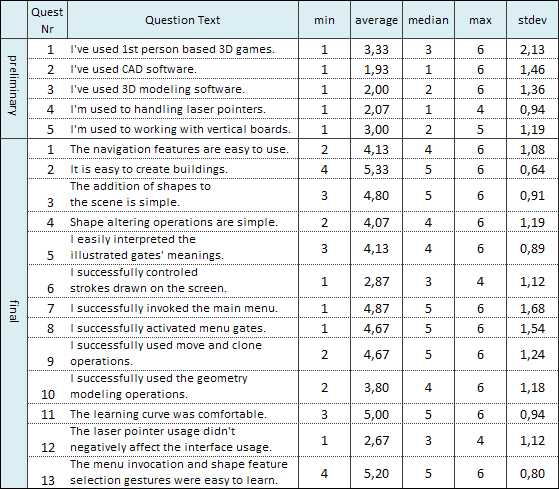
\includegraphics[width=0.8\columnwidth]{gfx/eval/table-questions18.png}
	\caption{Preliminary and Final Questionnaire close-ended questions and results}
	\label{table-questions18}
\end{table}

\begin{table}[htb]
	\centering
	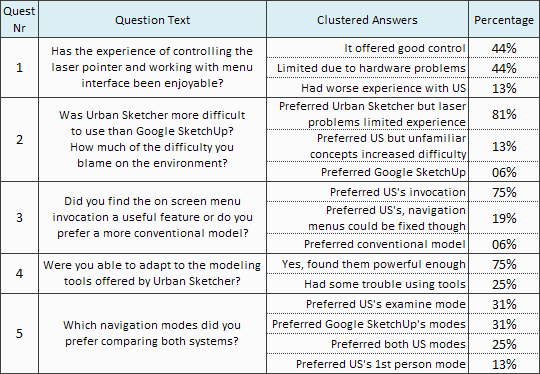
\includegraphics[width=0.8\columnwidth]{gfx/eval/table-questions5.png}
	\caption{Final Questionnaire open-ended questions and clustered answers}
	\label{table-questions5}
\end{table}

\begin{figure}[htb]
	\centering
	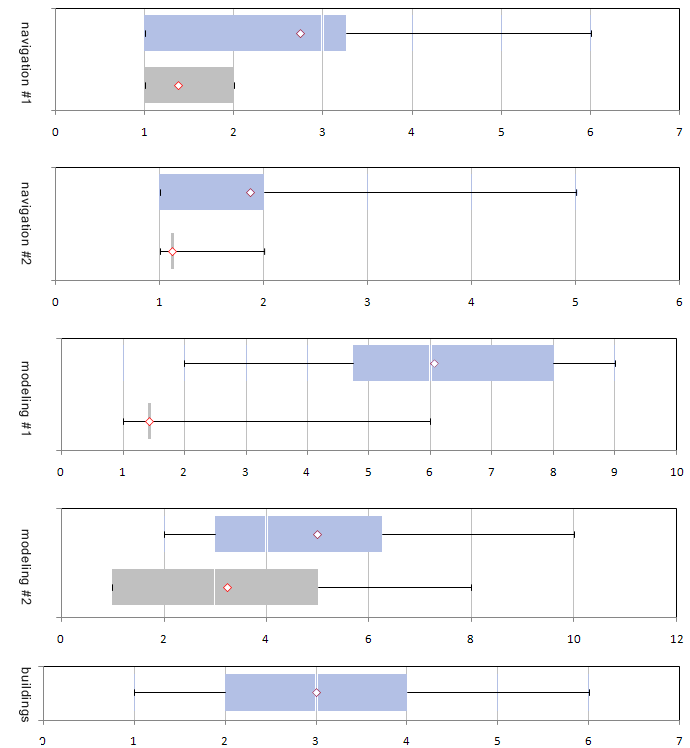
\includegraphics[width=0.8\columnwidth]{gfx/eval/bw-times2.png}
	\caption{Box and whiskers charts comparing task completion times on both systems}
	\label{graph-comparison}
\end{figure}


%\begin{figure}[htb]
%	\centering
%	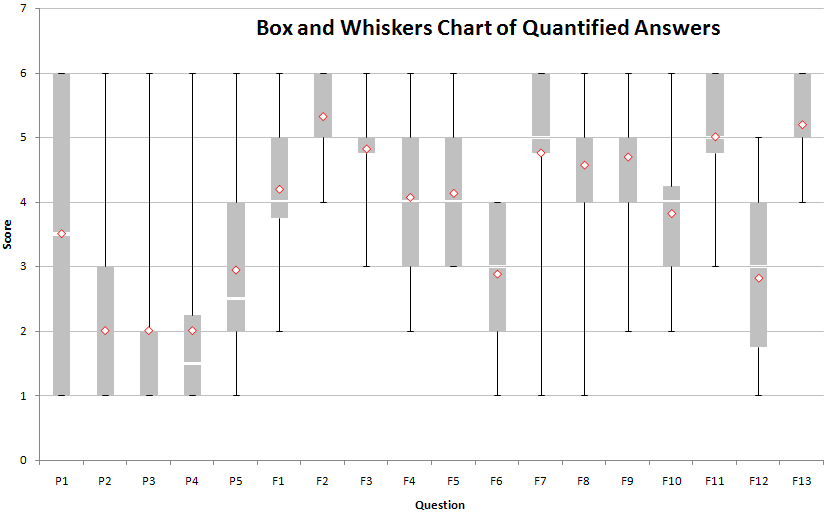
\includegraphics[width=\columnwidth]{gfx/eval/bw-questions.png}
%	\caption{Box and whiskers charts illustrating close-ended answers}
%	\label{graph-quantified}
%\end{figure}




%\begin{figure}[htb]
%	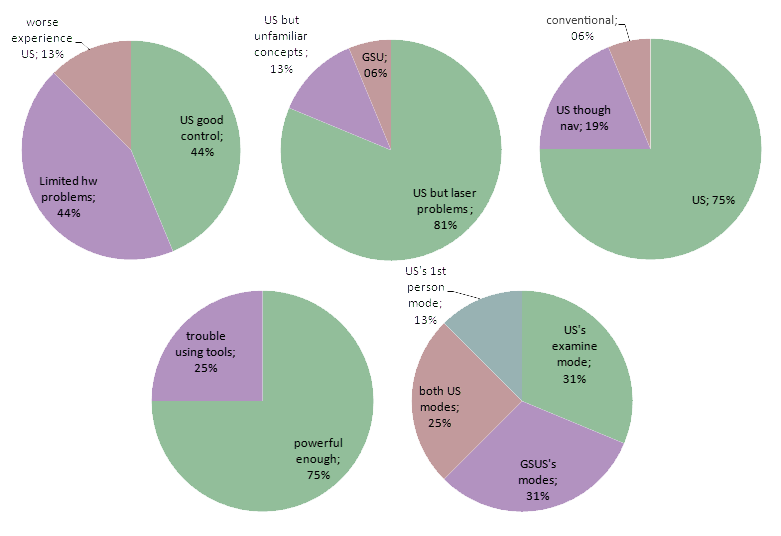
\includegraphics[width=\columnwidth]{gfx/eval/graph-pies.png}
%	\caption{Pie charts illustrating the clustered open-ended answers}
%	\label{graph-pies}
%\end{figure}


%\subsection{Discussion}

% US vs GSO - tempos, diferen�as, issues

%\subsubsection{Task Performance and Issues}

When looking at the time it took users to complete the tasks,
Urban Sketcher took between 50\% and 83\% more time than Google SketchUp.
This difference is small given that users performed Urban Sketcher tasks standing up,
using a novel user interface and handling a laser pointer on a limited tracking area.

The navigation tasks were the first to perform, with users getting acquainted with the interface.
Some undesired context menus were invoked at these first tasks, probably due to users drawing too fast.
When this happens, the laser tracking module segments the real strokes into small segments, misleading the system into recognizing these events as context menu invocations.

It was on the modeling tasks that differences between the systems were less notable.
This can be imputed to the carefully crafted modeling operations and their menus.
Some users took more time grasping the concept of stroke-long operations and their requirement to
keep the stroke active after triggering the operation to set its direction and length.
The main menu stroke gesture (a closed triangle) had worse recognition success rate on these operations.
This might have to do with users performing more context menu invocations and temporarily forgetting the correct
gesture to invoke the main menu or drawing triangles more roughly.

The building creation task was performed very smoothly in regard to its complexity.
Only a small set of individual problems occurred and users felt satisfied by the ease at
which they instanced buildings and assets.


%\subsubsection{Close-ended Answers Analysis}

% perguntas fechadas - 1o mais certas, depois mais favor�veis
The familiarity of users with 3D software and CAD proved to be low and the usage of 3D first person games disparate (P3, P2, P1).
Few users were used to handling laser pointers and some of them used vertical boards occasionally
-- this might be explained by the presence of two teachers on the user test (P4, P5).

Users found navigation, creation of buildings and shape creation and modeling fairly easy (F1, F2, F3, F4).
The illustrated gates were given a good recognition ratio and their activation was successful (F5).
Menu invocation and shape feature selection were easy to learn (F7, F8).
Both the move and clone operations were credited as functional and the learning curve classified comfortable (F9, F11).

Users diverged the most when asked about the success rate at which they controlled their strokes (F6).
This problem can be credited to laser tracking limitations on both tracked screen area and slow capturing frequency.
These originated visual deviations between real stroke and its interpretation, especially notable near the tracking boundaries.
Due to the slow capturing frequency, strokes had to be drawn slowly, otherwise they'd get segmented.
This problem was emphasized when performing apply-to-scene operations such as re-centering the examine center of interest or instancing new shapes which required continuity of stroke.


%\subsubsection{Open-ended Answers Analysis}

Most users held the laser tracking facilities responsible for some dissatisfaction and slowness in performing the tasks
when comparing with Google SketchUp (81\% of the users).
13\% of the users felt the novel interface unfamiliar therefore harder to master for a novice user while only 6\% elected
Google SketchUp as the best interface.
94\% of the users enjoyed the capacity of invoking menus as needed -- of these, 13\% pointed out that the navigation menu
could be fixed to the screen due to its constant usage, though this screen allocation problem was result solely of the
limited tracked area of screen -- if all screen was being tracked the menu could have remained there the whole time.
Out of all the users, only 25\% state having trouble with the modeling tools. This is satisfactory since many users
have shown low confidence at first when asked to perform the modeling tasks, ending up completing them with success and
reasserting their beliefs regarding such tasks. Several users felt this interface could be very effective on several domains
for controlling large screen displays.

It was shown that a stroke-based interface is capable of offering a set of complex actions and navigation modes to novice users
with them successfully performing tasks in reasonable time frames. Most users identified the laser tracking input as an obstacle
to an even better experience. This is a technical limitation which doesn't invalidate the application of these concepts and
interface with other technologies such as large multi touch surfaces.

\section{Conclusions and Future Work}

% motivation

The author designed and implemented a system named Urban Sketcher,
whose purpose is to provide architects and average users a way of making good use of large scale displays
for the creation of urban sceneries. Users can navigate the scene using several modes,
create and edit content such as buildings and custom shapes and review the scene by attaching notes to surfaces.
The system was implemented as a distributed modular application.
It was designed to support collaborative usage and laser pointers were used as main input device.
A novel user interface was devised, controlled by stroke input, with gestures, circular menus, area crossing activation 
(extending the work of \cite{CROSSY}).
The interface supports also multimodal modes -- speech commands and arm tracking were used to offer an alternate
way of moving the scene -- the multimodal flight mode. 
A building creation method was developed to provide a faster way
of generating buildings based on their style, described by a custom XML format
for describing fa�ade appearance, ceiling and shape details layout.
The set of provided tools for shape modeling proved sufficient for modeling simple shapes,
with users figuring out many creative ways of obtaining the requested shapes.



%\subsection{Results}

% RESULTS
The system was tested on several occasions for validation of navigation modes,
the multimodal mode and the building and modeling tools.
Since there's no clear contender in this area,
tests were conducted by comparing tasks performed by users
on Urban Sketcher on a large screen display against the same tasks
performed on Google SketchUp on a regular computer with keyboard and mouse input.
Users enjoyed working with the system and their performance completing the tasks
was at the most 50\% slower when comparing to their results on SketchUp,
an exciting result given the differences between both systems.
Users were introduced to a new way of input, a novel user interface and a set
of supported features uncommon to desktop software.
The stroke-based interface and menus proved capable on large screen environments
and the building creation and shape modeling features were learned and used efficiently.


% aplicabilidade

%\subsection{Main Contributions}

% u s concepts
This project introduced a new way of instantiating buildings using two strokes
-- one for defining the style and construction plane and the other to set the 
blueprint and facade height dimensions.
The architecture styles set can be enriched by users, with the system supporting
a custom XML format to define their layout and characteristics.

% custom shapes
In cases where custom 3D shapes are needed to enhance a particular aspect
of a building, users have the ability to creating custom shapes.
These can be edited by a small set of face and edge operations,
crafted to cover the most common needs of geometry modeling.
The most useful directions are estimated and made available for the user to manipulate the shape's
faces and edges, without the overhead of dozens of menu commands and parameters.
%so common in nowadays 3D modeling software.
Shapes can also be generated from other 3D applications such as the Blender 3D Modeler,
for which an exporter plug-in was generated, allowing the integration of externally created 3D content
into the system's internal shape format.

% gates e menus
To minimize the limitations of using laser pointers for interaction,
the gate concept was enhanced and applied.
Gates provide a way of users to activate options by drawing strokes over areas instead of clicking.
A non-intrusive menu form was defined and applied, with a minimalistic approach
at the starting interface, letting the users invoke and position menus as they see fit.
Complex operations were designed by activating the proper sequence of gates and interacting with
the scene in the stroke lifetime. Example of these is
shape instantiation by dropping it from a menu into the 3D view;
defining a building style and dimensions in two strokes time.

% navigation modes
A set of navigational modes was developed to cover the most common repositioning 
and tasks.
The popular first person mode was made available to give users the
possibility of exploring the scene as real users would. 
The compass navigation mode allows for seeing a top-down view of the nearby map,
allowing dragging the map for movement and  rotating the orientation
via a ring showing the cardinal points.
The examine navigation mode provides an effective way of inspecting an object of any
scale by moving around it. The examined object can also be easily changed.
Having a motion tracking capable system installed, one can also fly using the arms and voice
in the multimodal flight mode, which has proven both pleasing and effective,
empowering the user of an alternative way to rotate, change the altitude and flight speed
by making use of continuous arm movements.


%%%%%%%%%%%%%%%%%%%

%\subsection{Conclusions and Future Work}

Since this project addresses several subjects, there's space for
improvement on various aspects.
%There is space for improvement in several aspects of the project,
%even more since it addresses so many areas.
% work flow
The integration of real terrain data into the system could be eased by
the direct support of height maps, topography maps and aerial photographies.
A work flow for the importing of such content is outlined.
Facade walls could support blueprints other than rectangles.
% realism
Lighting conditions could be manipulated inside the program with an
accurate simulation of daylight, a subject highly valued
by architects for the definition of the location a building is to be built.
Textures and materials could make usage of the latest developments in GPU
technology to better convey the appearance of metal, glass and other materials.
%Techniques such as displacement or bump maps could be applied to offer greater depth to facade details.
% modeling operations
A more elaborate set of operations could be supported for modeling custom shapes.
%Most operations could be generalized for application to a group of edges or faces.
Even so, the available operations are a good compromise between the complexity
of professional modelers and the stroke-based, minimalistic interface provided.
Given the state of the art on large screen displays and input technologies for them,
this project successfully made use of laser pointers and a cluster of projectors
to deliver both a comprehensive interface based on strokes and a building prototyping
application for it. Users managed to complete simple navigation and modeling tasks along
with building manipulation with reasonable performance times.


% aplica��es

%\section{Possible Applications}

Urban Sketcher is an application using the underlying system for the purpose of creating urban scenarios,
but other fields could benefit from its features.
The system would be a good starting point for the development of an interactive whiteboard for teaching.
It could be further extended for collaborative exploration and reviewing scenarios.
Given its modular framework, laser pointers could also be replaced by multi-touch surfaces as input device,
a trend gaining momentum and being applied to an ever growing set of systems.
The replacement of lasers by the touch surface would increase the accuracy of the strokes due to the
proximity of user finger and screen. The increased sampling frequency would also improve the Kalman Filter's
success in asserting which user owns each stroke. Most of the user interface work keep relevancy with such
input device, such as stroke gestures to call menus, the menu functionality itself and gate usage.

This project spawned a number of novel interaction concepts, offering a way of modeling custom shapes and
buildings according to predetermined styles and explore the virtual world using several navigation modes.
Most of the interaction concepts developed here can be applied to emerging technologies such as multi-touch
surfaces.
The project's architecture proved robust and users got along with the system, its concepts and interface.


\bibliographystyle{plain}
\bibliography{dissertation} 

\end{document}
